\documentclass{standalone}
\usepackage{tikz}
\usetikzlibrary{patterns, positioning}
\usepackage[sfdefault]{ClearSans} %% option 'sfdefault' activates Clear Sans as the default text font
\usepackage[T1]{fontenc}

\begin{document}
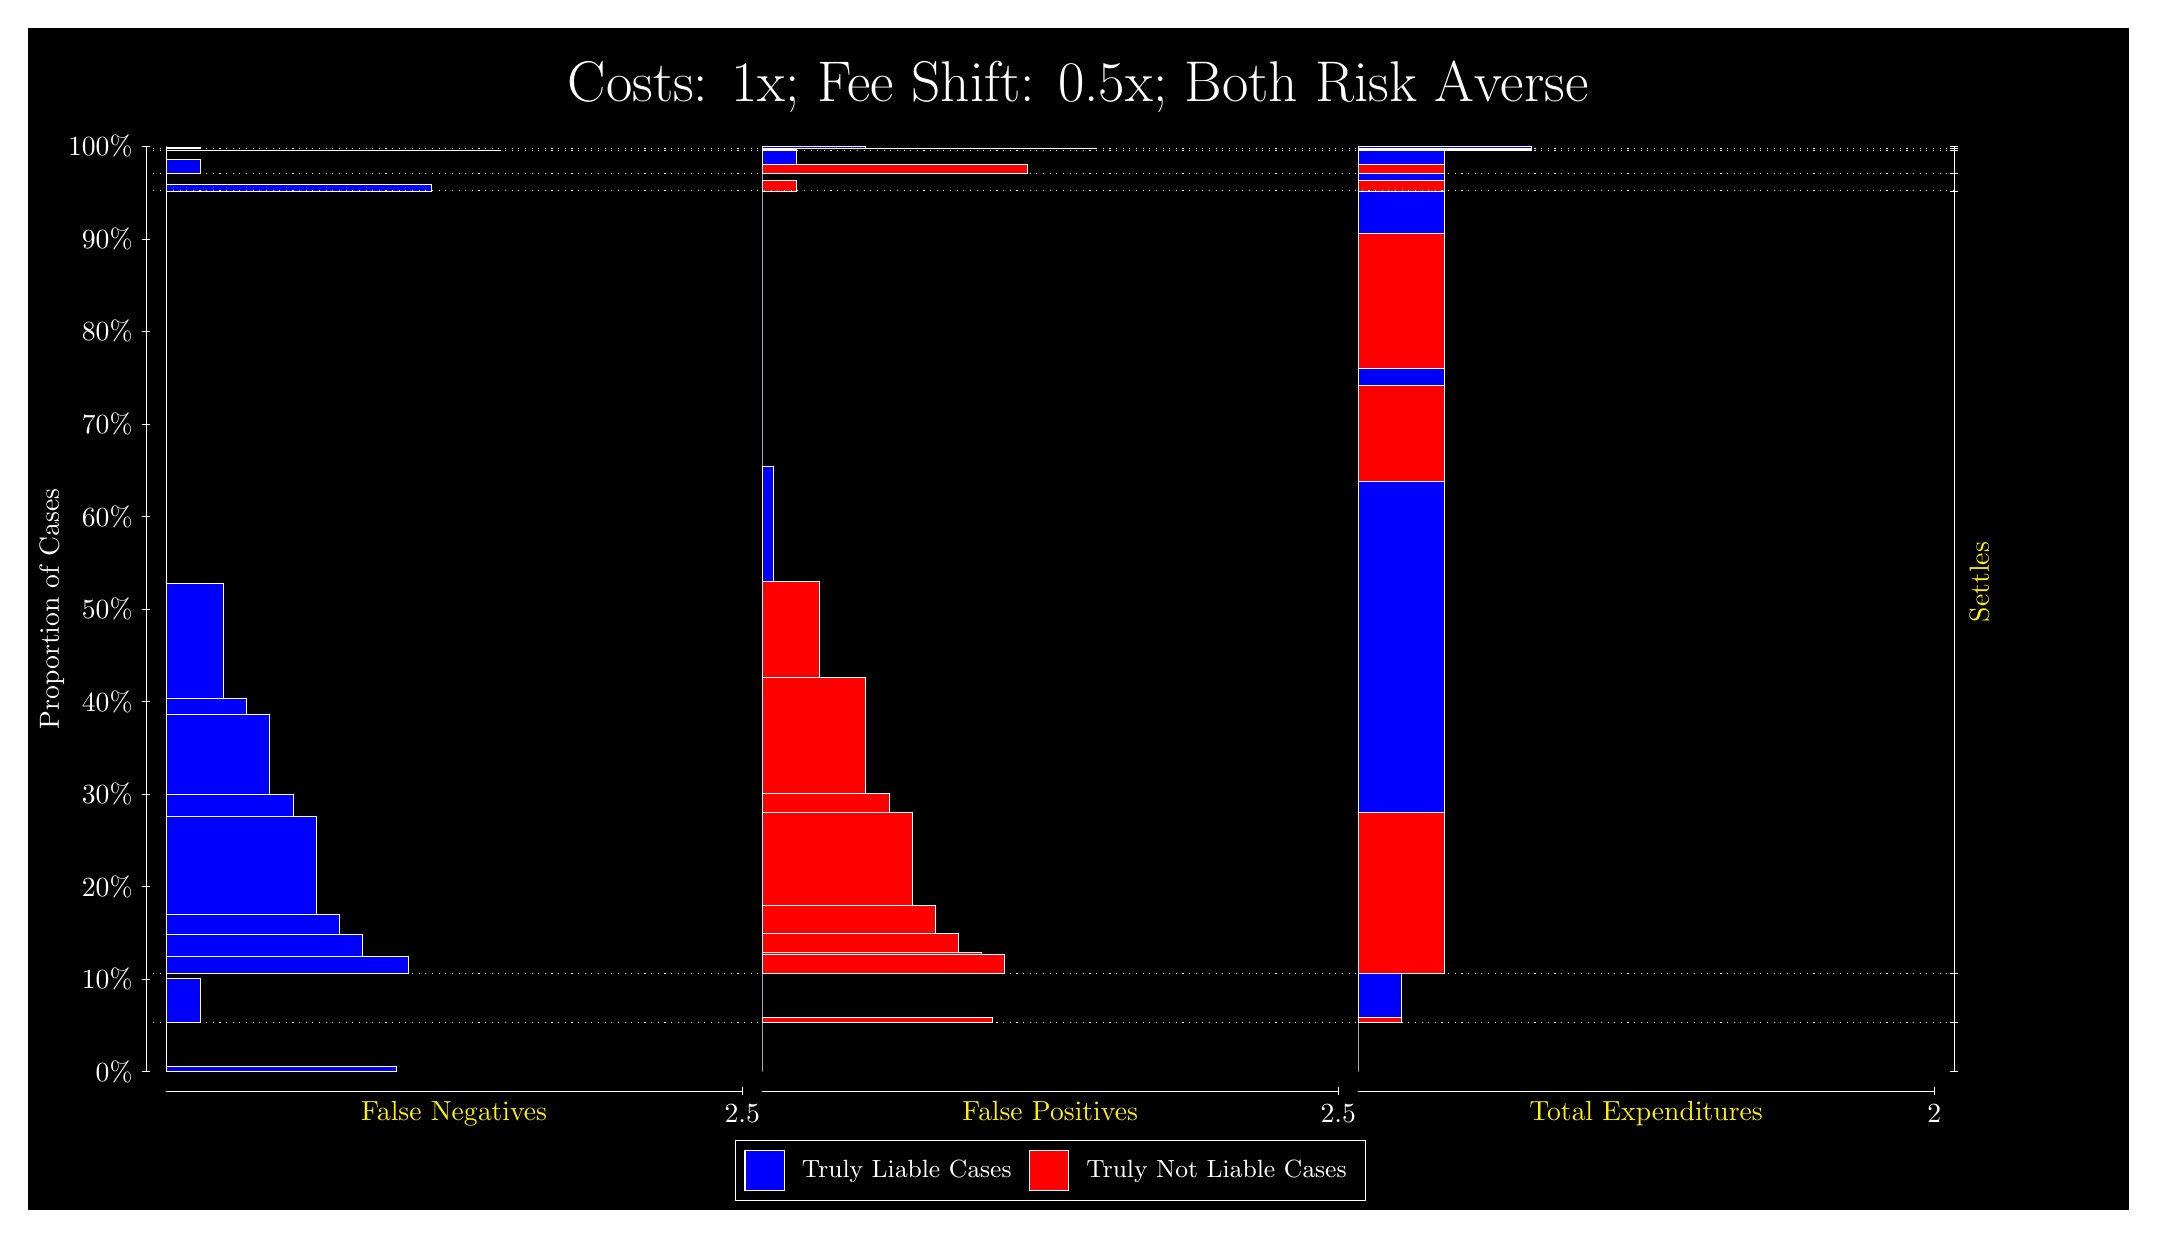
\begin{tikzpicture}
\draw[fill=black] (0,0) rectangle (26.667,15);
\draw[text=white] (0,13.5) rectangle (26.667,15) node[midway] {\huge Costs: 1x; Fee Shift: 0.5x; Both Risk Averse};
\draw[white, very thin] (1.5,1.75) -- (1.5,13.5);
\node[rotate=90, text=white, anchor=center] at (0.3, 7.625) {Proportion of Cases};
\draw[white, very thin] (1.45,1.75) -- (1.55,1.75);
\node[text=white, anchor=east] at (1.45, 1.75) {0\%};
\draw[white, very thin] (1.45,2.925) -- (1.55,2.925);
\node[text=white, anchor=east] at (1.45, 2.925) {10\%};
\draw[white, very thin] (1.45,4.1) -- (1.55,4.1);
\node[text=white, anchor=east] at (1.45, 4.1) {20\%};
\draw[white, very thin] (1.45,5.275) -- (1.55,5.275);
\node[text=white, anchor=east] at (1.45, 5.275) {30\%};
\draw[white, very thin] (1.45,6.45) -- (1.55,6.45);
\node[text=white, anchor=east] at (1.45, 6.45) {40\%};
\draw[white, very thin] (1.45,7.625) -- (1.55,7.625);
\node[text=white, anchor=east] at (1.45, 7.625) {50\%};
\draw[white, very thin] (1.45,8.8) -- (1.55,8.8);
\node[text=white, anchor=east] at (1.45, 8.8) {60\%};
\draw[white, very thin] (1.45,9.975) -- (1.55,9.975);
\node[text=white, anchor=east] at (1.45, 9.975) {70\%};
\draw[white, very thin] (1.45,11.15) -- (1.55,11.15);
\node[text=white, anchor=east] at (1.45, 11.15) {80\%};
\draw[white, very thin] (1.45,12.325) -- (1.55,12.325);
\node[text=white, anchor=east] at (1.45, 12.325) {90\%};
\draw[white, very thin] (1.45,13.5) -- (1.55,13.5);
\node[text=white, anchor=east] at (1.45, 13.5) {100\%};

\draw[white, very thin] (24.457,1.75) -- (24.457,13.5);
\draw[white, very thin] (24.407,1.75) -- (24.507,1.75);
\node[anchor=west] at (24.407, 1.75) {};
\draw[white, very thin] (24.407,2.3747) -- (24.507,2.3747);
\node[anchor=west] at (24.407, 2.3747) {};
\draw[white, very thin] (24.407,2.9993) -- (24.507,2.9993);
\node[anchor=west] at (24.407, 2.9993) {};
\draw[white, very thin] (24.407,12.935) -- (24.507,12.935);
\node[anchor=west] at (24.407, 12.935) {};
\draw[white, very thin] (24.407,13.157) -- (24.507,13.157);
\node[anchor=west] at (24.407, 13.157) {};
\draw[white, very thin] (24.407,13.446) -- (24.507,13.446);
\node[anchor=west] at (24.407, 13.446) {};
\draw[white, very thin] (24.407,13.472) -- (24.507,13.472);
\node[anchor=west] at (24.407, 13.472) {};
\draw[white, very thin] (24.407,13.5) -- (24.507,13.5);
\node[anchor=west] at (24.407, 13.5) {};

\draw[white, very thin, fill=blue] (1.75,1.75) rectangle (4.6775,1.8157);
\draw[white, very thin, fill=red] (1.75,1.8157) rectangle (1.75,2.3747);
\draw[white, very thin, fill=blue] (1.75,2.3747) rectangle (2.1891,2.9336);
\draw[white, very thin, fill=red] (1.75,2.9336) rectangle (1.75,2.9993);
\draw[white, very thin, fill=blue] (1.75,2.9993) rectangle (4.8239,3.2089);
\draw[white, very thin, fill=blue] (1.75,3.2089) rectangle (4.2384,3.4981);
\draw[white, very thin, fill=blue] (1.75,3.4981) rectangle (3.9457,3.7493);
\draw[white, very thin, fill=blue] (1.75,3.7493) rectangle (3.6529,4.9892);
\draw[white, very thin, fill=blue] (1.75,4.9892) rectangle (3.3602,5.2754);
\draw[white, very thin, fill=blue] (1.75,5.2754) rectangle (3.0674,6.2931);
\draw[white, very thin, fill=blue] (1.75,6.2931) rectangle (2.7746,6.4918);
\draw[white, very thin, fill=blue] (1.75,6.4918) rectangle (2.4819,7.9548);
\draw[white, very thin, fill=red] (1.75,7.9548) rectangle (1.75,12.935);
\draw[white, very thin, fill=blue] (1.75,12.935) rectangle (5.1167,13.022);
\draw[white, very thin, fill=red] (1.75,13.022) rectangle (1.75,13.157);
\draw[white, very thin, fill=blue] (1.75,13.157) rectangle (2.1891,13.337);
\draw[white, very thin, fill=red] (1.75,13.337) rectangle (1.75,13.446);
\draw[white, very thin, fill=blue] (1.75,13.446) rectangle (5.9949,13.455);
\draw[white, very thin, fill=red] (1.75,13.455) rectangle (1.75,13.472);
\draw[white, very thin, fill=blue] (1.75,13.472) rectangle (2.1891,13.491);
\draw[white, very thin, fill=red] (1.75,13.491) rectangle (1.75,13.5);
\draw[white, very thin, fill=red] (9.3189,1.75) rectangle (9.3189,2.3089);
\draw[white, very thin, fill=blue] (9.3189,2.3089) rectangle (9.3189,2.3747);
\draw[white, very thin, fill=red] (9.3189,2.3747) rectangle (12.246,2.4404);
\draw[white, very thin, fill=blue] (9.3189,2.4404) rectangle (9.3189,2.9993);
\draw[white, very thin, fill=red] (9.3189,2.9993) rectangle (12.393,3.2359);
\draw[white, very thin, fill=red] (9.3189,3.2359) rectangle (12.1,3.2674);
\draw[white, very thin, fill=red] (9.3189,3.2674) rectangle (11.807,3.5006);
\draw[white, very thin, fill=red] (9.3189,3.5006) rectangle (11.515,3.8637);
\draw[white, very thin, fill=red] (9.3189,3.8637) rectangle (11.222,5.0389);
\draw[white, very thin, fill=red] (9.3189,5.0389) rectangle (10.929,5.281);
\draw[white, very thin, fill=red] (9.3189,5.281) rectangle (10.636,6.7577);
\draw[white, very thin, fill=red] (9.3189,6.7577) rectangle (10.051,7.9794);
\draw[white, very thin, fill=blue] (9.3189,7.9794) rectangle (9.4652,9.4424);
\draw[white, very thin, fill=blue] (9.3189,9.4424) rectangle (9.3189,12.935);
\draw[white, very thin, fill=red] (9.3189,12.935) rectangle (9.758,13.07);
\draw[white, very thin, fill=blue] (9.3189,13.07) rectangle (9.3189,13.157);
\draw[white, very thin, fill=red] (9.3189,13.157) rectangle (12.686,13.266);
\draw[white, very thin, fill=blue] (9.3189,13.266) rectangle (9.758,13.446);
\draw[white, very thin, fill=red] (9.3189,13.446) rectangle (9.758,13.463);
\draw[white, very thin, fill=blue] (9.3189,13.463) rectangle (9.3189,13.472);
\draw[white, very thin, fill=red] (9.3189,13.472) rectangle (13.564,13.481);
\draw[white, very thin, fill=blue] (9.3189,13.481) rectangle (10.636,13.5);
\draw[white, very thin, fill=red] (16.888,1.75) rectangle (16.888,2.3089);
\draw[white, very thin, fill=blue] (16.888,2.3089) rectangle (16.888,2.3747);
\draw[white, very thin, fill=red] (16.888,2.3747) rectangle (17.437,2.4404);
\draw[white, very thin, fill=blue] (16.888,2.4404) rectangle (17.437,2.9993);
\draw[white, very thin, fill=red] (16.888,2.9993) rectangle (17.986,5.0389);
\draw[white, very thin, fill=blue] (16.888,5.0389) rectangle (17.986,9.2444);
\draw[white, very thin, fill=red] (16.888,9.2444) rectangle (17.986,10.466);
\draw[white, very thin, fill=blue] (16.888,10.466) rectangle (17.986,10.676);
\draw[white, very thin, fill=red] (16.888,10.676) rectangle (17.986,12.395);
\draw[white, very thin, fill=blue] (16.888,12.395) rectangle (17.986,12.935);
\draw[white, very thin, fill=red] (16.888,12.935) rectangle (17.986,13.07);
\draw[white, very thin, fill=blue] (16.888,13.07) rectangle (17.986,13.157);
\draw[white, very thin, fill=red] (16.888,13.157) rectangle (17.986,13.266);
\draw[white, very thin, fill=blue] (16.888,13.266) rectangle (17.986,13.446);
\draw[white, very thin, fill=red] (16.888,13.446) rectangle (19.083,13.463);
\draw[white, very thin, fill=blue] (16.888,13.463) rectangle (19.083,13.472);
\draw[white, very thin, fill=red] (16.888,13.472) rectangle (19.083,13.481);
\draw[white, very thin, fill=blue] (16.888,13.481) rectangle (19.083,13.5);
\draw[white, dotted] (1.5,2.3747) -- (24.457,2.3747);
\draw[white, dotted] (1.5,2.9993) -- (24.457,2.9993);
\draw[white, dotted] (1.5,12.935) -- (24.457,12.935);
\draw[white, dotted] (1.5,13.157) -- (24.457,13.157);
\draw[white, dotted] (1.5,13.446) -- (24.457,13.446);
\draw[white, dotted] (1.5,13.472) -- (24.457,13.472);
\draw[white, very thin] (1.75,1.5) -- (9.0689,1.5);
\node[text=yellow, anchor=north] at (5.4094, 1.5) {False Negatives};
\draw[white, very thin] (9.0689,1.45) -- (9.0689,1.55);
\node[text=white, anchor=north] at (9.0689, 1.45) {2.5};

\draw[white, very thin] (9.3189,1.5) -- (16.638,1.5);
\node[text=yellow, anchor=north] at (12.978, 1.5) {False Positives};
\draw[white, very thin] (16.638,1.45) -- (16.638,1.55);
\node[text=white, anchor=north] at (16.638, 1.45) {2.5};

\draw[white, very thin] (16.888,1.5) -- (24.207,1.5);
\node[text=yellow, anchor=north] at (20.547, 1.5) {Total Expenditures};
\draw[white, very thin] (24.207,1.45) -- (24.207,1.55);
\node[text=white, anchor=north] at (24.207, 1.45) {2};



\node[text=yellow, centered, rotate=90] at (24.777, 7.9671) {Settles};





\draw (12.978300999999998,1.5) node[draw=none] (baseCoordinate) {};
\begin{scope}[align=center]
        \matrix[scale=0.5, draw=white, below=0.5cm of baseCoordinate, nodes={draw}, column sep=0.1cm]{
            \node[rectangle, draw, minimum width=0.5cm, minimum height=0.5cm, fill=blue] {}; &
            \node[draw=none, font=\small, text=white] (B) {Truly Liable Cases}; &
            \node[rectangle, draw, minimum width=0.5cm, minimum height=0.5cm, fill=red] {}; &
            \node[draw=none, font=\small, text=white] (B) {Truly Not Liable Cases}; \\
            };
\end{scope}

\end{tikzpicture}
\end{document}